\documentclass[12pt,a4paper]{article}
\usepackage[utf8]{inputenc}
\usepackage{amsmath,amssymb,amsfonts,amsthm}
\usepackage{geometry}
\geometry{margin=1in}
\usepackage{graphicx}
\usepackage{hyperref}
\usepackage{fancyhdr}
\usepackage{tikz}
\usetikzlibrary{decorations.markings, arrows.meta}
\usepackage{setspace}
\usepackage{parskip}

% Custom colors for links and styling
\usepackage{xcolor}
\definecolor{primaryblue}{RGB}{0, 51, 102}
\definecolor{secondaryblue}{RGB}{51, 153, 255}

\hypersetup{
    colorlinks=true,
    linkcolor=primaryblue,
    filecolor=magenta,      
    urlcolor=cyan,
    pdftitle={Complex Conformal Mappings},
    pdfpagemode=FullScreen,
    pageanchor=false
}

% Header and Footer Setup
\pagestyle{fancy}
\fancyhf{}
\renewcommand{\headrulewidth}{0pt}
\cfoot{\thepage}

\newtheorem{theorem}{Theorem}[section]
\newtheorem{definition}{Definition}[section]

\begin{document}
\pagenumbering{gobble}

% ===== Front Page (Page 1) =====
\begin{titlepage}
    \centering
    % BHU Header Logo
    
\includegraphics[width=0.78\textwidth]{bhu_logo.png} \\[1.8em]

    % University Name & Location
    {\fontsize{18}{22}\selectfont \textbf{BANARAS HINDU UNIVERSITY}} \\[0.4em]
    {\large Varanasi, Uttar Pradesh, India} \\[3.5em]

    % Report Title & Subtitle
    {\fontsize{22}{28}\selectfont \textbf{Study of Complex Conformal Mappings}} \\[0.6em]
    {\large \textbf{Theoretical Overview, Standard Transformations, and Applications}} \\[1.2em]
    {\Large \textit{Internship Project Report}} \\[3.5em]

    % Degree / Program Info
    {\large \textit{B.Sc. (Hons.) Mathematics}}

    \vfill

    % Details Section: Submitted By (Left) and Guided By (Right)
    \noindent
    \begin{minipage}[t]{0.55\textwidth}
        \raggedright
        \textbf{Submitted By:}\\[0.4em]
        Aryan Maurya\\[0.2em]
        Roll No.: 24220MAT051\\[0.2em]
        Enrolment No.: 476633\\[0.3em]
        Department of Mathematics
    \end{minipage}%
    \begin{minipage}[t]{0.45\textwidth}
        \raggedleft
        \textbf{Guided By:}\\[0.4em]
        Dr. Pravati Sahoo\\[0.2em]
        Associate Professor\\[0.3em]
        Department of Mathematics,\\
        MMV, BHU
    \end{minipage}

    \vspace{3.5em}

    % Date Section
    \begin{center}
        Date: 31 July 2026
    \end{center}
\end{titlepage}


% ===== Declaration Page (Page 3) =====
\begin{center}
    {\Large \textbf{DECLARATION}}
\end{center}

\vspace{1.2cm}

\setstretch{1.4}
\large

\noindent I, \textbf{Aryan Maurya}, student of B.Sc (4\textsuperscript{th} Semester) Roll No. \textbf{24220MAT051}, do hereby certify that the project work titled “\textbf{Study of Complex Conformal Mappings: Theoretical Overview, Standard Transformations, and Applications}” is a bonafide work carried out by me.

\vspace{2cm}

\noindent Date: 31 July 2026 \\[1.5em]
\noindent Place: Varanasi

\vspace{2.5cm}

\noindent
\begin{minipage}[t]{0.5\textwidth}
    Signature of the Candidate:\\[2.5em]
    Name:
\end{minipage}%
\begin{minipage}[t]{0.5\textwidth}
    \raggedleft
    \textbf{Dr. Pravati Sahoo}\\[0.3em]
    Department of Mathematics\\[0.3em]
    MMV, Banaras Hindu University\\[2em]
    (Signature and Stamp)
\end{minipage}

\clearpage

% ===== Acknowledgement Page (Page 4) =====
\begin{center}
    {\Large \textbf{ACKNOWLEDGEMENT}}
\end{center}

\vspace{0.8cm}

\setstretch{1.25}

I would like to express my sincere gratitude and deep sense of reverence to my esteemed guide, \textbf{Dr. Pravati Sahoo}, Associate Professor, Department of Mathematics, Mahila Maha Vidyalaya (MMV), Banaras Hindu University, for her invaluable guidance, constant encouragement, and insightful feedback throughout the course of my internship. Her profound knowledge, constructive suggestions, and academic support were instrumental in the successful completion of this report titled \textit{“Study of Complex Conformal Mappings: Theoretical Overview, Standard Transformations, and Applications”}.

I extend my heartfelt thanks to the \textbf{Department of Mathematics, MMV, BHU} and the \textbf{Institute of Science, Banaras Hindu University}, for providing the necessary academic infrastructure, learning environment, and resources required for this two-week internship program.

I am also grateful to all the faculty members, staff, and research scholars of the Department of Mathematics for their cooperation and indirect assistance during the period of my internship.

Finally, I would like to express my sincere appreciation to my family and friends for their constant motivation, understanding, and moral support throughout my academic endeavors.

\vspace{1.5cm}

\begin{flushright}
    \setstretch{1.1}
    \textbf{Aryan Maurya}\\
    B.Sc. Semester IV\\
    Examination Roll No.: 24220MAT051\\
    Institute of Science\\
    Banaras Hindu University, Varanasi
\end{flushright}

\clearpage
\restoregeometry
\pagestyle{fancy}
\hypersetup{pageanchor=true}

% ===== Table of Contents =====
\pagenumbering{roman}
\tableofcontents
\newpage

% ===== Main Content =====
\pagenumbering{arabic}

\section{Introduction}
\subsection{Historical Background}
The origins of conformal mapping trace back to the field of cartography and geography in the 16th and 18th centuries. The Mercator projection, presented by Gerardus Mercator in 1569, was the first widely used map projection that preserved angles locally, allowing navigators to plot straight courses of constant compass bearing. In the mid-18th century, Leonhard Euler and Joseph-Louis Lagrange laid the mathematical foundations for conformal mappings in two dimensions during their studies of geographic maps.

The field was revolutionized in the 19th century by Bernhard Riemann. In his landmark 1851 doctoral dissertation, Riemann formulated the geometric theory of functions of a complex variable and introduced the Riemann Mapping Theorem, establishing that any simply connected domain in the complex plane (other than the plane itself) can be mapped conformally onto the unit disk. Subsequently, Hermann Amandus Schwarz and Elwin Bruno Christoffel independently developed the Schwarz-Christoffel formula in the late 1860s, providing a systematic way to construct conformal maps from the upper half-plane to arbitrary polygonal domains.

\subsection{Mathematical Definition and Overview}
In mathematics, a \textbf{conformal mapping} (or conformal transformation) is a function that preserves angles locally. This means that if two curves intersect at a point in the domain, the angle between their tangent lines at the point of intersection is preserved in both magnitude and orientation (direction) in the image domain.

Let $U$ and $V$ be open subsets of the complex plane $\mathbb{C}$. A mapping $w = f(z)$ from $U$ to $V$ is conformal at a point $z_0 \in U$ if for any two smooth curves $\gamma_1, \gamma_2$ intersecting at $z_0$, the angle between their tangents at $z_0$ is equal to the angle between the tangents of the mapped curves $f(\gamma_1), f(\gamma_2)$ at $w_0 = f(z_0)$.

\begin{theorem}
A complex-valued function $f(z) = u(x,y) + iv(x,y)$ is conformal at $z_0$ if and only if it is analytic (holomorphic) at $z_0$ and its derivative is non-zero, i.e., $f'(z_0) \neq 0$.
\end{theorem}

\section{Mathematical Formulation}
\subsection{The Cauchy-Riemann Equations}
For a complex function $f(z) = u(x,y) + iv(x,y)$ to be analytic in a domain $D$, it must satisfy the Cauchy-Riemann equations:
\begin{equation}
    \frac{\partial u}{\partial x} = \frac{\partial v}{\partial y} \quad \text{and} \quad \frac{\partial u}{\partial y} = -\frac{\partial v}{\partial x}
\end{equation}
When these equations are satisfied and the partial derivatives are continuous, the function $f(z)$ is differentiable. If $f'(z) \neq 0$, the Jacobian matrix of the transformation:
\begin{equation}
    J = \begin{pmatrix}
        u_x & u_y \\
        v_x & v_y
    \end{pmatrix} = \begin{pmatrix}
        u_x & -v_x \\
        v_x & u_x
    \end{pmatrix}
\end{equation}
represents a rotation scaling matrix. The determinant of the Jacobian is:
\begin{equation}
    \det(J) = u_x^2 + v_x^2 = |f'(z)|^2 > 0
\end{equation}
Since $\det(J) > 0$ and the matrix is a scalar multiple of an orthogonal matrix, it preserves angles and orientation, which is the defining property of a conformal map.

\subsection{Angle Preservation (Geometric Proof)}
Let $z(t) = x(t) + iy(t)$ be a curve in the $z$-plane passing through $z_0$ at $t = 0$. The tangent vector to the curve at $z_0$ is given by $z'(0)$. Under the mapping $w = f(z)$, the image curve is $w(t) = f(z(t))$. By the chain rule:
\begin{equation}
    w'(0) = f'(z_0) \cdot z'(0)
\end{equation}
Taking the argument (angle) of both sides:
\begin{equation}
    \arg(w'(0)) = \arg(f'(z_0)) + \arg(z'(0))
\end{equation}
This indicates that the tangent vector of the mapped curve is rotated by an angle of $\alpha = \arg(f'(z_0))$ and scaled by $|f'(z_0)|$, regardless of the direction of the curve. Therefore, any two curves intersecting at $z_0$ will both be rotated by the same angle $\alpha$, preserving the relative angle between them in both magnitude and orientation.

\subsection{Necessary and Sufficient Conditions for Conformality}
Based on the geometric properties of complex derivatives, we can establish the conditions under which a transformation $w = f(z)$ represents a conformal mapping:
\begin{enumerate}
    \item \textbf{Necessary Condition:} If $w = f(z)$ represents a conformal mapping of a domain $D$ in the $z$-plane into a domain $D'$ in the $w$-plane, then $f(z)$ must be an analytic (holomorphic) function of $z$ in $D$.
    \item \textbf{Sufficient Condition:} If $f(z)$ is an analytic function of $z$ in a domain $D$ and its derivative is non-zero ($f'(z) \neq 0$) inside $D$, then the mapping $w = f(z)$ is conformal at all points of $D$.
\end{enumerate}
Under a conformal transformation $w = f(z)$, the tangent at $z_0$ to any curve passing through $z_0$ is rotated through an angle $\theta_0 = \arg(f'(z_0))$, and the distance of any point in the neighborhood of $z_0$ is scaled (magnified) by the factor $|f'(z_0)|$.

\section{Classification and Types of Conformal Mappings}
Conformal transformations can be classified based on several criteria: their behavior regarding angle orientation, the dimensionality of the space in which they act, their global domain of definition, and generalizations that allow for bounded angle distortion.

\subsection{Classification by Orientation (Direct vs. Indirect / Conformal vs. Isogonal)}
Let a point $P(x_0, y_0)$ in the $z$-plane be mapped to $P'(u_0, v_0)$ in the $w$-plane, and let two curves $C_1, C_2$ intersecting at $P$ be mapped to curves $\Gamma_1, \Gamma_2$ intersecting at $P'$. We classify these mappings based on how they treat the angle between the curves:
\begin{description}
    \item[\textbf{Conformal Mapping (Direct Conformal):}] The mapping is said to be conformal at $P$ if the angle between the tangent lines of $\Gamma_1$ and $\Gamma_2$ at $P'$ is equal to the angle between the tangent lines of $C_1$ and $C_2$ at $P$, both in \textbf{magnitude} and in \textbf{sense (direction of rotation)}. A complex function $w = f(z)$ is conformal at a point if and only if it is holomorphic (analytic) and its derivative is non-zero ($f'(z) \neq 0$).
    \item[\textbf{Isogonal Mapping (Indirect Conformal / Orientation-Reversing):}] The mapping is said to be isogonal at $P$ if the angle between the tangent lines of the mapped curves preserves the \textbf{magnitude} of the original angle but reverses the \textbf{sense of rotation}. In complex analysis, indirect conformal mappings are represented by anti-holomorphic functions of the form $w = f(\overline{z})$, where $f$ is holomorphic and $f'(z) \neq 0$. The most basic example is complex conjugation, $w = \overline{z}$ (which represents reflection across the real axis).
\end{description}

\subsection{Classification by Space Dimension (Liouville's Rigidity)}
The nature and variety of conformal mappings differ dramatically depending on the dimension $n$ of the Euclidean space $\mathbb{R}^n$:
\begin{itemize}
    \item \textbf{Two-Dimensional (2D) Conformal Mappings ($n = 2$):} In the complex plane, there is an infinite-dimensional space of conformal mappings. Any non-constant holomorphic function is locally conformal wherever its derivative is non-zero. This provides immense flexibility, allowing conformal mapping of arbitrary simply connected domains (Riemann Mapping Theorem).
    \item \textbf{Higher-Dimensional Conformal Mappings ($n \ge 3$):} In contrast to the 2D case, conformal mappings in dimensions 3 and higher are extremely rigid. By Liouville's Theorem on Conformal Rigidity, the only conformal maps on domains in $\mathbb{R}^n$ ($n \ge 3$) are combinations of:
    \begin{enumerate}
        \item \textit{Translations:} $x \mapsto x + a$
        \item \textit{Rotations / Orthogonal Transformations:} $x \mapsto R x$ (where $R \in O(n)$)
        \item \textit{Dilations / Scaling:} $x \mapsto \lambda x$ (where $\lambda > 0$)
        \item \textit{Inversions in spheres:} $x \mapsto \frac{x - x_0}{|x - x_0|^2}$
    \end{enumerate}
    These generate the finite-dimensional M\"obius group in higher dimensions.
\end{itemize}

\subsection{Classification by Domain Scope (Local vs. Global)}
Mappings can be conformal locally without being globally one-to-one:
\begin{itemize}
    \item \textbf{Local Conformal Mappings:} A function $f(z)$ is locally conformal at $z_0$ if it is conformal in a small neighborhood around $z_0$. For example, $w = z^2$ is conformal at all points in $\mathbb{C}$ except the origin ($z = 0$). However, it is not globally conformal on $\mathbb{C}$ because it is not one-to-one (e.g., $f(1) = f(-1) = 1$).
    \item \textbf{Global Conformal Mappings (Conformal Automorphisms):} A mapping is globally conformal if it is a conformal bijection from a domain $\Omega$ onto itself or another domain. For example, the M\"obius transformations map the Riemann sphere $\hat{\mathbb{C}}$ conformally and bijectively to itself.
\end{itemize}

\subsection{Generalization: Quasi-conformal Mappings}
In many physical applications, strict conformality is too restrictive. A \textbf{quasi-conformal mapping} is a generalization that allows for a bounded amount of angle distortion. Geometrically, instead of mapping infinitesimal circles to infinitesimal circles (as conformal mappings do), quasi-conformal mappings map infinitesimal circles to infinitesimal ellipses with a bounded eccentricity (ratio of major to minor axes). They satisfy the Beltrami equation:
\begin{equation}
    \frac{\partial f}{\partial \overline{z}} = \mu(z) \frac{\partial f}{\partial z}
\end{equation}
where $|\mu(z)| \le k < 1$. When $\mu(z) = 0$, this reduces to the Cauchy-Riemann equations, and the mapping becomes strictly conformal.

\subsection{Ordinary and Critical Points}
To characterize the conformality of a mapping at specific points, we define:
\begin{itemize}
    \item \textbf{Ordinary Points:} A point $z_0$ where the function $f(z)$ is analytic and its derivative is non-zero and finite ($0 < |f'(z_0)| < \infty$) is called an ordinary point. At every ordinary point, the mapping $w = f(z)$ is conformal.
    \item \textbf{Critical Points:} A point $z_0$ where the derivative $f'(z_0) = 0$ or $f'(z_0) = \infty$ is called a critical point. At critical points, the mapping fails to be conformal.
\end{itemize}
For a Möbius transformation $w = \frac{az+b}{cz+d}$ ($ad - bc \neq 0$), the derivative is:
\begin{equation}
    \frac{dw}{dz} = \frac{ad - bc}{(cz + d)^2}
\end{equation}
This derivative becomes infinite at $z = -d/c$ and vanishes at $z = \infty$. Thus, the critical points of a Möbius transformation are $z = -d/c$ and $z = \infty$. At these points, conformality does not hold, whereas all other points in the complex plane are ordinary (conformal) points.

\section{Important Theorems in Conformal Mapping}
Conformal mappings are governed by deep topological and analytical properties. Below are some of the most fundamental theorems in the field.

\begin{theorem}[The Riemann Mapping Theorem]
Let $\Omega$ be a simply connected open subset of the complex plane $\mathbb{C}$ which is not equal to $\mathbb{C}$ itself. Then there exists a unique bijective, analytic mapping $f(z)$ from $\Omega$ onto the open unit disk $\mathbb{D} = \{w \in \mathbb{C} : |w| < 1\}$ such that for a given $z_0 \in \Omega$, $f(z_0) = 0$ and $f'(z_0) > 0$.
\end{theorem}
This theorem is remarkable because it guarantees that any simply connected region, no matter how geometrically complicated (such as a jagged snowflake shape or a narrow polygon), can be mapped conformally and bijectively to a perfect unit disk.

\begin{theorem}[Schwarz Reflection Principle]
Let $\Omega$ be a symmetric domain with respect to the real axis, and let $\Omega^+$ be the portion of $\Omega$ lying in the upper half-plane. Let $f(z)$ be a continuous function on $\Omega^+ \cup (\Omega \cap \mathbb{R})$, analytic on $\Omega^+$, such that $f(z)$ is real whenever $z \in \Omega \cap \mathbb{R}$. Then $f(z)$ can be analytically continued to the entire domain $\Omega$ by defining:
\begin{equation}
    f(z) = \overline{f(\overline{z})} \quad \text{for } z \in \Omega^-
\end{equation}
Furthermore, this extension remains conformal on $\Omega$.
\end{theorem}
This principle allows mathematicians and physicists to extend conformal mappings from a half-plane or symmetric region across straight-line boundaries.

\begin{theorem}[Open Mapping Theorem]
If $f(z)$ is a non-constant holomorphic function on a connected open set $U \subset \mathbb{C}$, then $f(U)$ is an open set. In particular, conformal maps are open mappings.
\end{theorem}

\begin{theorem}[Liouville's Theorem on Conformal Rigidity]
For dimensions $n \ge 3$, any conformal mapping on a domain of the Euclidean space $\mathbb{R}^n$ is composed of translations, rotations, dilations, and inversions (i.e., it must be a M\"obius transformation).
\end{theorem}
This theorem highlights the exceptional status of two-dimensional complex analysis. In 2D, the class of conformal mappings is infinite-dimensional and incredibly flexible, whereas in 3D and higher, it is extremely rigid and restricted.

\section{Standard Mappings and Illustrative Examples}
Here we explore some of the most common conformal mappings, their geometric behavior, and their analytical properties.

\subsection{M\"obius Transformations}
A M\"obius transformation (also known as a bilinear or fractional linear transformation) is defined as:
\begin{equation}
    w = f(z) = \frac{az + b}{cz + d}
\end{equation}
where $a, b, c, d \in \mathbb{C}$ and $ad - bc \neq 0$.
\begin{itemize}
    \item \textbf{Properties:} Möbius transformations map circles and lines to circles and lines. They set up a one-to-one conformal mapping of the entire closed $z$-plane onto the closed $w$-plane, making them biuniform.
    \item \textbf{Derivative:} $f'(z) = \frac{ad - bc}{(cz + d)^2}$, which is non-zero everywhere except at the critical point $z = -d/c$.
\end{itemize}

\subsubsection{Decomposition of Möbius Transformations}
Every Möbius transformation is the resultant of the four elementary geometric transformations: translation, rotation, magnification, and inversion. This can be proved by decomposition:
\begin{itemize}
    \item \textbf{Case 1 ($c \neq 0$):} We can rewrite $w$ as:
    \begin{equation}
        w = \frac{a}{c} + \frac{bc - ad}{c^2 \left( z + d/c \right)}
    \end{equation}
    This can be broken down into the following sequence of elementary transformations:
    \begin{enumerate}
        \item \textit{Translation} by $d/c$: $Z_1 = z + \frac{d}{c}$
        \item \textit{Inversion}: $Z_2 = \frac{1}{Z_1}$
        \item \textit{Rotation and Magnification} by $\frac{bc - ad}{c^2}$: $Z_3 = \left(\frac{bc - ad}{c^2}\right) Z_2$
        \item \textit{Translation} by $a/c$: $w = Z_3 + \frac{a}{c}$
    \end{enumerate}
    \item \textbf{Case 2 ($c = 0$):} Since $ad - bc \neq 0$, we must have $d \neq 0$. The mapping reduces to a linear transformation:
    \begin{equation}
        w = \frac{a}{d}z + \frac{b}{d}
    \end{equation}
    which is decomposed as:
    \begin{enumerate}
        \item \textit{Rotation and Magnification} by $a/d$: $Z_1 = \left(\frac{a}{d}\right) z$
        \item \textit{Translation} by $b/d$: $w = Z_1 + \frac{b}{d}$
    \end{enumerate}
    In this case, no inversion is required.
\end{itemize}

\subsection{The Cayley Transform (Example \& Theorem)}
The Cayley transform is a specific M\"obius transformation that maps the upper half-plane to the unit disk.
\begin{theorem}
The mapping $w = f(z) = \frac{z - i}{z + i}$ is a conformal bijection from the upper half-plane $\mathbb{H} = \{z \in \mathbb{C} : \text{Im}(z) > 0\}$ to the open unit disk $\mathbb{D} = \{w \in \mathbb{C} : |w| < 1\}$.
\end{theorem}
\begin{proof}
Let $z = x + iy$ with $y > 0$. We want to show that $|w| < 1$.
\begin{equation}
    |w|^2 = \left| \frac{z - i}{z + i} \right|^2 = \frac{|x + i(y-1)|^2}{|x + i(y+1)|^2} = \frac{x^2 + (y-1)^2}{x^2 + (y+1)^2}
\end{equation}
Since $y > 0$, we have $(y-1)^2 = y^2 - 2y + 1 < y^2 + 2y + 1 = (y+1)^2$. Hence, the numerator is strictly less than the denominator, meaning $|w| < 1$. The boundary of the half-plane (the real axis $\mathbb{R}$) maps to the boundary of the unit disk (the circle $|w| = 1$), and $z = i$ maps to $w = 0$.
\end{proof}

\subsection{Geometric Inversion and Inverse Points}
The standard mapping $w = 1/z$ is closely related to the geometric concept of inversion with respect to a circle.
\begin{definition}[Inverse Points]
Let $\gamma$ be a circle of radius $R$ and center $c$ in the complex plane. Two points $a$ and $b$ are said to be inverse points with respect to the circle $\gamma$ if they lie on the same ray originating from $c$ and the product of their distances from the center satisfies:
\begin{equation}
    |a - c| \cdot |b - c| = R^2
\end{equation}
In complex coordinates, the relation is:
\begin{equation}
    (a - c)\overline{(b - c)} = R^2 \quad \implies \quad b = c + \frac{R^2}{\overline{a} - \overline{c}}
\end{equation}
Furthermore, if the circle is represented in general coordinates as:
\begin{equation}
    A z\overline{z} + \alpha z + \overline{\alpha}\overline{z} + C = 0 \quad (\text{where } A, C \in \mathbb{R}, \alpha \in \mathbb{C})
\end{equation}
then two points $z$ and $z'$ are inverse points if and only if they satisfy:
\begin{equation}
    A z\overline{z'} + \alpha z + \overline{\alpha}\overline{z'} + C = 0
\end{equation}
\end{definition}

If the circle is the unit circle $|z| = 1$ (centered at the origin $c = 0$ with radius $R = 1$, corresponding to $A=1$, $\alpha=0$, $C=-1$), the inverse point of $z$ is:
\begin{equation}
    z' = \frac{1}{\overline{z}}
\end{equation}
The inversion mapping $w = 1/z$ can therefore be written as:
\begin{equation}
    w = \frac{1}{z} = \overline{\left( \frac{1}{\overline{z}} \right)} = \overline{z'}
\end{equation}
This formulation shows that the mapping $w = 1/z$ is the product of two transformations:
\begin{enumerate}
    \item A geometric inversion in the unit circle: $z \mapsto z' = 1/\overline{z}$ (which preserves angle magnitude but reverses orientation, hence isogonal).
    \item A reflection in the real axis: $z' \mapsto \overline{z'} = w$ (which also reverses orientation, hence isogonal).
\end{enumerate}
Because both individual mappings are isogonal (orientation-reversing), their composition preserves orientation, making the mapping $w = 1/z$ conformal.

\subsection{The Exponential Mapping \texorpdfstring{$w = e^z$}{w = e\textasciicircum z}}
The exponential function $f(z) = e^z = e^{x}(\cos y + i\sin y)$ maps:
\begin{itemize}
    \item Vertical lines $x = c_1$ to circles $|w| = e^{c_1}$.
    \item Horizontal lines $y = c_2$ to rays $\arg(w) = c_2$.
\end{itemize}
It is conformal everywhere since $f'(z) = e^z \neq 0$.

\subsection{The Power Mapping \texorpdfstring{$w = z^n$}{w = z\textasciicircum n}}
For $n \ge 2$, the mapping $w = z^n$ is conformal everywhere except at $z = 0$, where $f'(0) = 0$. At the origin, angles are multiplied by $n$.

\subsection{The Joukowsky Transform (Example \& Theorem)}
The Joukowsky transform is a famous conformal mapping used in aeronautical engineering.
\begin{theorem}
The mapping $w = f(z) = z + \frac{1}{z}$ is conformal for all $z \neq 0$ and $z \neq \pm 1$. It maps circles in the $z$-plane to aerodynamic shapes called airfoils in the $w$-plane.
\end{theorem}
\begin{proof}
We find the derivative:
\begin{equation}
    f'(z) = 1 - \frac{1}{z^2}
\end{equation}
Thus, the mapping is conformal everywhere except at the critical points $z = \pm 1$ and the pole $z = 0$. In polar coordinates $z = re^{i\theta}$:
\begin{equation}
    w = re^{i\theta} + \frac{1}{r}e^{-i\theta} = \left( r + \frac{1}{r} \right)\cos\theta + i \left( r - \frac{1}{r} \right)\sin\theta
\end{equation}
For the unit circle $r = 1$, the imaginary part vanishes, mapping the entire circle to the line segment $[-2, 2]$ on the real axis. However, if we shift the circle slightly in the $z$-plane so that it passes through $z = 1$ and contains $z = -1$ in its interior, the image under $f(z)$ is a streamlined closed curve resembling a cross-section of an airplane wing.
\end{proof}

\section{Visualizing Conformal Mappings}
Below is a conceptual visualization of how a rectangular grid in the $z$-plane is mapped conformal-wise under a transformation like $w = z^2$ or $w = e^z$.

\begin{figure}[h!]
    \centering
    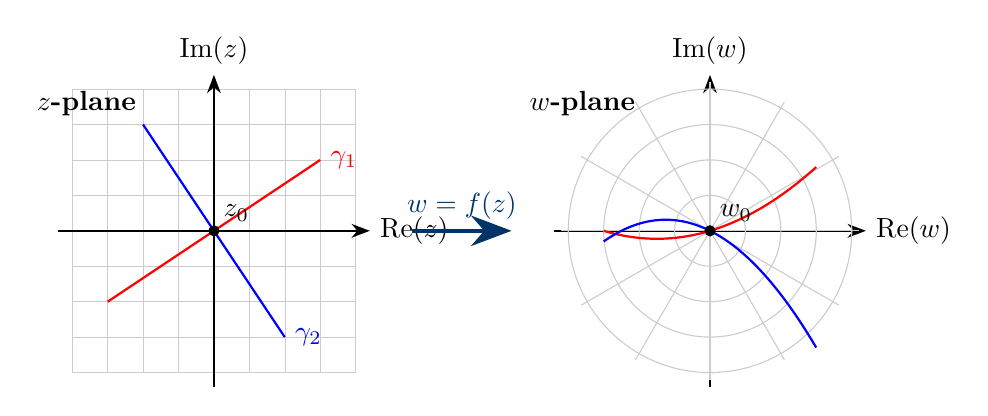
\begin{tikzpicture}[scale=0.9]
        % Z-plane grid
        \begin{scope}[shift={(0,0)}]
            \draw[step=0.5cm,gray!40,very thin] (-2,-2) grid (2,2);
            \draw[-{Stealth},thick] (-2.2,0) -- (2.2,0) node[right] {Re($z$)};
            \draw[-{Stealth},thick] (0,-2.2) -- (0,2.2) node[above] {Im($z$)};
            \node at (-1.8, 1.8) {\textbf{$z$-plane}};
            
            % Draw two intersecting lines
            \draw[red, thick] (-1.5,-1) -- (1.5,1) node[right] {$\gamma_1$};
            \draw[blue, thick] (-1,1.5) -- (1,-1.5) node[right] {$\gamma_2$};
            \filldraw[black] (0,0) circle (2pt) node[above right] {$z_0$};
        \end{scope}
        
        % Mapping Arrow
        \draw[-{Stealth[scale=1.5]},line width=1.5pt,primaryblue] (2.8,0) -- (4.2,0) node[midway,above] {$w = f(z)$};
        
        % W-plane grid (conformal curves)
        \begin{scope}[shift={(7,0)}]
            \draw[-{Stealth},thick] (-2.2,0) -- (2.2,0) node[right] {Re($w$)};
            \draw[-{Stealth},thick] (0,-2.2) -- (0,2.2) node[above] {Im($w$)};
            \node at (-1.8, 1.8) {\textbf{$w$-plane}};
            
            % Draw conformal grid (concentric circles and rays)
            \foreach \r in {0.5,1.0,1.5,2.0} {
                \draw[gray!40, thin] (0,0) circle (\r);
            }
            \foreach \a in {0,30,60,90,120,150,180,210,240,270,300,330} {
                \draw[gray!40, thin] (0,0) -- (\a:2.1);
            }
            
            % Intersecting mapped curves showing preserved angle
            \draw[red, thick, domain=-1.5:1.5, samples=100] plot (\x, {0.2*\x*\x + 0.3*\x});
            \draw[blue, thick, domain=-1.5:1.5, samples=100] plot (\x, {-0.4*\x*\x - 0.5*\x});
            \filldraw[black] (0,0) circle (2pt) node[above right] {$w_0$};
        \end{scope}
    \end{tikzpicture}
    \caption{Visualizing angle preservation and conformal grids under transformation.}
\end{figure}

\section{Real-Life Use Cases and Applications}
Conformal mapping is a vital mathematical tool in physics, engineering, geography, and computer science due to its unique property of preserving local angles and transforming Laplace's equation ($\nabla^2 \phi = 0$) into simpler domains.

\subsection{Cartography and Navigation}
The most widespread application of conformal mapping is in map projections. The \textbf{Mercator projection} is a conformal mapping from the sphere (representing Earth) to a cylinder. Because it preserves angles, a straight line drawn on a Mercator map corresponds to a line of constant compass bearing (a rhumb line). This property made it the standard for maritime navigation and remains the basis for modern web mapping applications such as Google Maps (Web Mercator).

\subsection{Aerodynamics and Aviation}
The design of early aircraft wings relied heavily on the \textbf{Joukowsky transformation} ($w = z + 1/z$). In fluid mechanics, finding the flow pattern around an intricate shape like a wing profile is highly complex. By mapping the wing profile to a perfect circle where the flow lines are simple concentric lines (using conformal mapping), engineers can compute lift, drag, and velocity profiles analytically. This solved lift coefficient equations before the advent of computational fluid dynamics (CFD).

\subsection{Electrical Engineering and Electrostatics}
In microelectronics and printed circuit board (PCB) design, engineers need to compute the capacitance and electric fields between conductors of irregular geometries. By finding a conformal map that transforms these shapes into parallel plates, the electric potential $\Phi$ (which satisfies Laplace's equation $\nabla^2 \Phi = 0$) can be computed easily. Since the composition of a harmonic function with an analytic function is still harmonic, the solution in the simple domain transforms directly back to the physical domain.

\subsection{Medical Imaging and Computer Graphics}
In modern computer graphics and medical imaging (such as brain mapping), 3D surfaces need to be mapped to 2D planes for texture mapping or analysis. Conformal parameterization is used to map 3D triangular meshes of organs (like the brain or heart) to a flat disk or sphere while minimizing distortion. By preserving local angles, the shapes of features are kept highly recognizable, which is critical for medical diagnostics.

\section{Conclusion}
Conformal mapping bridges complex analysis and real-world physical systems. This report highlights the mathematical core, properties, standard maps, important theorems, and real-life engineering utility of conformal transformations. Future research will explore numerical conformal mapping using Schwartz-Christoffel formulas.

\newpage
\section{References}
The following standard textbooks, widely prescribed in Indian universities for undergraduate and postgraduate courses in Complex Analysis, have been used as primary references for this report:

\begin{enumerate}
    \item \textbf{Functions of a Complex Variable} by \textit{J.N. Sharma}. \\
    S. Chand \& Company, New Delhi. \textit{(Chapters: Conformal Mapping, Bilinear Transformations)}

    \item \textbf{Theory of Functions of a Complex Variable} by \textit{Shanti Narayan \& P.K. Mittal}. \\
    S. Chand \& Company, New Delhi. \textit{(Chapters: Analytic Functions, Conformal Mappings)}

    \item \textbf{Complex Variables and Applications} by \textit{R.V. Churchill \& J.W. Brown}. \\
    McGraw-Hill Education. \textit{(Chapters: Conformal Mapping, Applications of Conformal Mapping)}
\end{enumerate}

\end{document}
